% !TEX spellcheck = en
\documentclass[main.tex]{subfiles} 

\begin{document}
%%%%%%%%%%%%%%%%%%%%%%%%%%%%%%%%%%%%%%%%%%%%%%%%%%%%%
%%%%%%%%%%%%%%%%%%%    Appendices   %%%%%%%%%%%%%%%%%%%%%%
%%%%%%%%%%%%%%%%%%%%%%%%%%%%%%%%%%%%%%%%%%%%%%%%%%%%%
\appendix

\section{Visualization of Vector Fields}
\label{sec:vis_vec_field}

\subsection{Notation}
%%%%%%%%%%%%     VECTOR FIELDS      %%%%%%%%%%%%
Vectors are a set of objects that exist in a \emph{vector space} $V$. On the vector space, 
there are defined two operations; addition and multiplication\footnote{Along with the axioms
that must hold for all vectors in $V$.}. The entire vector space is spanned by the orthogonal 
basis vectors. 

\begin{mydef}
Let the orthoganal basis $\{\hat{e}_1,\hat{e}_2,\hat{e}_3\}$ span vector space V,
then a linear combination of the bases represent a vector $\mathbf{v}$ in $\mathbf{R}^3$.
In component form, the vector is given as
\begin{align} \label{eq:comp_form}
\mathbf{v} = v_1\hat{e}_1 + v_2\hat{e}_2 + v_3\hat{e}_3.
\end{align}
\end{mydef}

\hspace{-6mm}The components of the vector $\mathbf{v}$ can be, for the sake of brevity, written 
as a tuple $(v_1,v_2,v_3)$ with the understanding\cite{Hei01} that we are refering to the component form 
\eqref{eq:comp_form}. Likewise, we can define a vector in $\mathbf{R}^N$, where the N components
in component form, are given as  $(v_1,\hdots,v_N)$. Dots imply the remaining components 
of the vector, instead of listing them all up. The vector space is spanned by the basis 
$\{\hat{e}_1,\hdots,\hat{e}_N\}$.
\\

The length of an N-dimensional vector is given by the Euclidean norm $\lVert{\mathbf{v}\rVert}$
\begin{align}
\label{euclidnorm}
\lVert{\mathbf{v}\rVert} = \sqrt{v_1^2 + \hdots + v_N^2} \hspace{1mm}.
\end{align}
Given a vector $\mathbf{v}$, we can normalize it by dividing it by it's own length
$\mathbf{v}/\lVert{\mathbf{v}\rVert}$. Such a normalized vector is called a \emph{unit vector}.
If a set of unit vectors are orthogonal to each other, then they are called \emph{orthonormal}.
If a set of orthonormal vectors span the entire vector space $V$, then such a set is called
\emph{orthonormal basis}. Unless we specify otherwise, all bases herein will be assumed 
to be orthonormal. 
\\

Assigning a vector to each point in a subset of space generates a \emph{vector field}. This 
requires a slightly different notation than Equation\eqref{eq:comp_form}. In order to assign 
a location for a vector $(v_1,v_2,v_3)$, we consider the components of the vector as a function 
of $\mathbf{x}$, where $\mathbf{x} = (x_1,x_2,x_3)$.
\begin{align*}
\mathbf{v} = v_1(\mathbf{x})\hat{e}_1 + v_2(\mathbf{x})\hat{e}_2 + v_3(\mathbf{x})\hat{e}_3.
\end{align*}
As with Equation\eqref{eq:comp_form}, we can extend this to N-dimensional vector spaces.
The vector components would then be functions of $\mathbf{x} = (x_1,\hdots,x_N)$. A simple 
vector field $(x,y,z)$ is displayed in Figure \ref{fig:vector_field_xyz}. Here, the magnitude of the 
vectors is displayed by color. As we would expect, for a cartesian coordinate system, the "intensity" 
of the field increases the further we get away from the origo.

\begin{figure}
\hspace{5mm}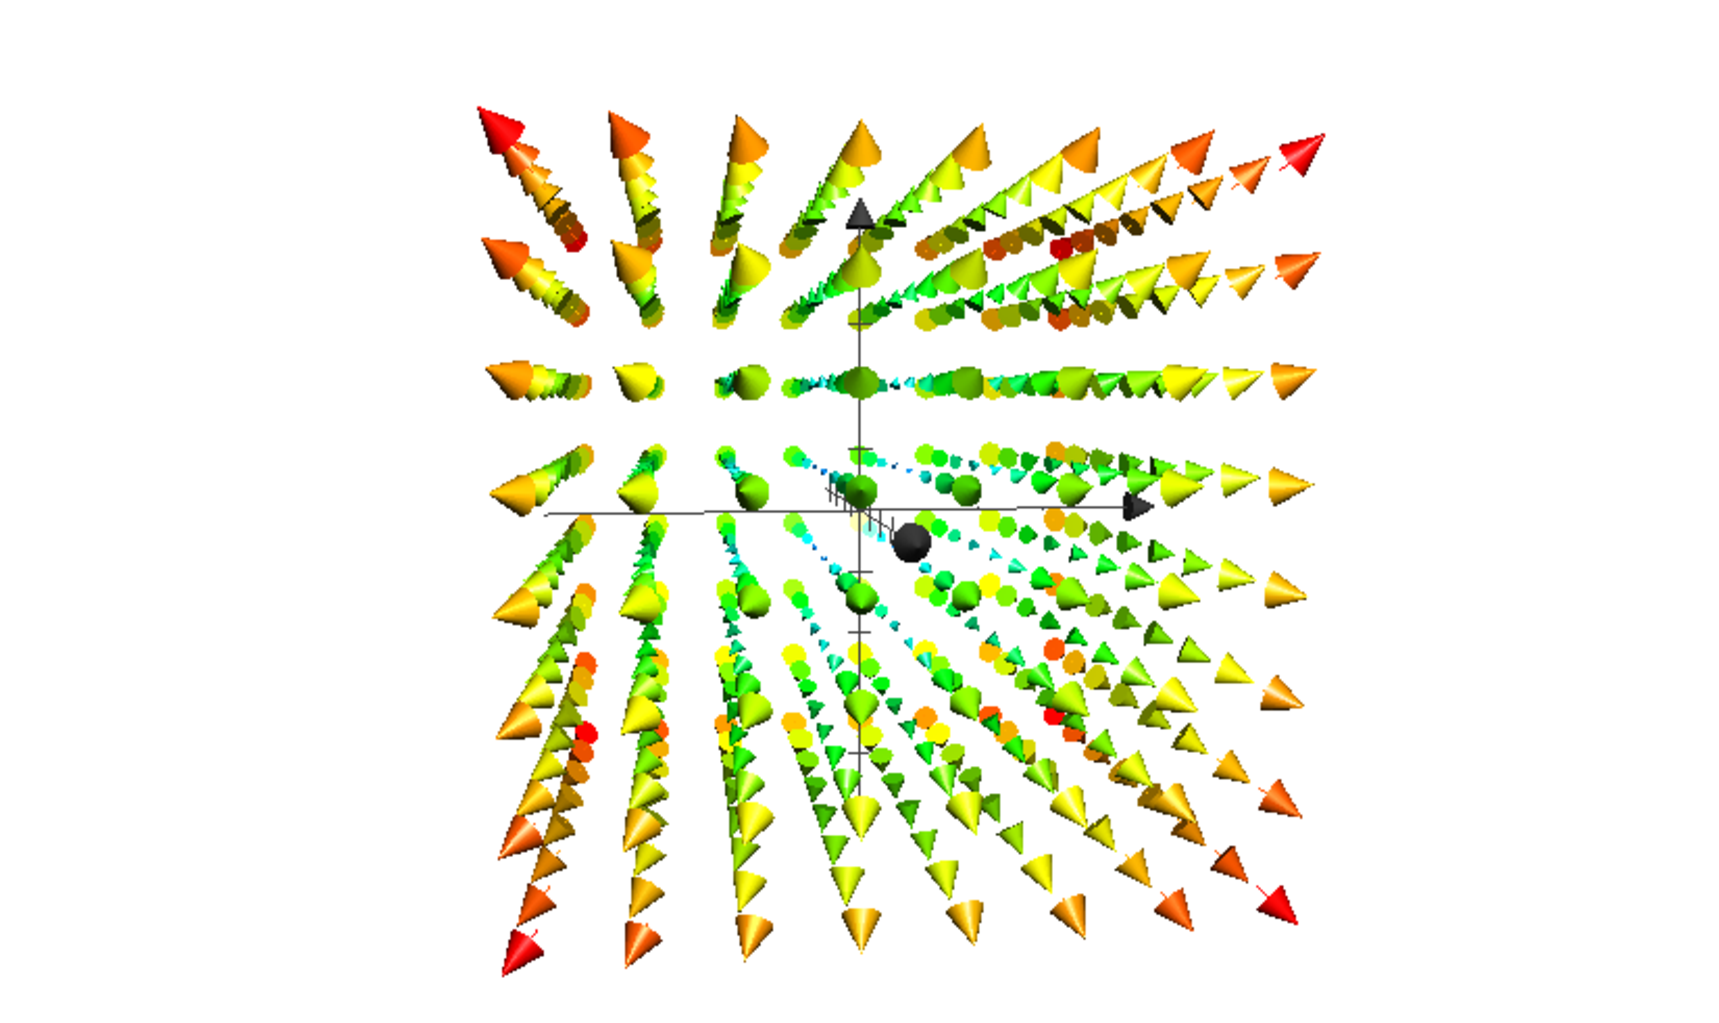
\includegraphics[scale=0.5,natwidth=29.11,natheight=17.33]{../figures/velocity_field_xyz.pdf} 
\caption{Vector field (x,y,z) displayed using a simple graphical tool in OS X.}
\label{fig:vector_field_xyz}
\end{figure}


%%%%%%%%%%%%     STREAMLINES      %%%%%%%%%%%%
\subsection{Streamlines}
Besides using vectors to display vector fields, another useful method is the displaying of streamlines.
\begin{mydef}
A Streamline is a curve where the vectors in a vector field are always tangent to the curve.
\end{mydef}

For a vector field we can display the movement of a given particle at any 
location in the vector field. If the vector field changes with time, i.e vector field is unsteady, 
then we freeze the time at an instaneous moment, and draw the streamlines. The streamline
is the path which the particle takes, or rather the path it must take as determined by the 
vector field at an instantaneous moment\footnote{For a steady field, the vector field never changes.
Hence the streamlines will thus remain constant.}. 
Mathematically, we can determine the path by solving the differential equations
\begin{align}
\left.\frac{dx_1}{v_1(\mathbf{x})}\right|_{t = t_0} 
= \left.\frac{dx_2}{v_2(\mathbf{x})}\right|_{t = t_0} 
= \left.\frac{dx_3}{v_3(\mathbf{x})}\right|_{t = t_0}
\end{align}
By integrating separably, these equations can be solved at any position $\mathbf{x}$ and a given
time $t = t_0$. 
\\

Numerically, this is accomplished by creating a grid for the vector field. Thereupon,
numerical integration is performed on the computational grid. Using for example the forward 
Euler scheme, we can advance the path which the particle takes by a user-defined step size. 
The process of solving the system of ODE (ordinary differential equations) by a finite difference 
method is as following. 

We start at a given point in the domain and allow the vector field to dictate in
which direction and to where we are to progress along. Hence, the path becomes the unknown 
quantity which we must determine. For $\mathbf{v} \in \mathbf{R}^2$, we can list the whole
process :
\begin{enumerate}
\item Discretize the domain \textbf{x}$\in$[0,{\large x}\textsubscript{max}]$\times$[0,{
\large y}\textsubscript{max}] where the vector field exists.
\item Use a start point ({\large x}\textsubscript{0},{\large y}\textsubscript{0}) 
to initiate the integration.
\item Perform forward and backward integration (depending on where you start in the domain).
\end{enumerate}
To perform the numerical integration, there are several numerical methods that can be employed.


\subsection{Numerical Integration}
The following algorithm lists all the necessary steps involved when performing numerical
integration
\begin{algorithm}[H]
\caption{Integration by forward Euler scheme} \label{alg:FE_Integration}
\begin{algorithmic}[1]
\State \textit{Load vector field data into arrays}
\State \textit{Create a grid over a domain for which the vector field exists upon}
\State \textit{Create arrays for storage of the streamline data}
\State \textit{Perform numerical integration by the forward Euler method}
\State \textit{Repeat process for backwards integration}
\State \textit{Stitch together all the entries for forward and backwards integration}
\end{algorithmic}
\end{algorithm}

The computational grid, defined at postion $(x_i,y_j)$, can be drawn as following
\begin{align*}
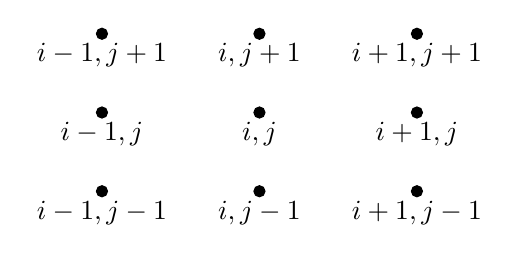
\begin{tikzpicture}
	\draw [fill] (-2,2) circle [radius=2pt] node[below]{$i-1,j+1$};
	\draw [fill] (0,2) circle [radius=2pt] node[below]{$i,j+1$};
	\draw [fill] (2,2) circle [radius=2pt] node[below]{$i+1,j+1$};
	\draw [fill] (-2,1) circle [radius=2pt] node[below]{$i-1,j$};
	\draw [fill] (0,1) circle [radius=2pt] node[below]{$i,j$};
	\draw [fill] (2,1) circle [radius=2pt] node[below]{$i+1,j$};
	\draw [fill] (-2,0) circle [radius=2pt] node[below]{$i-1,j-1$};
	\draw [fill] (0,0) circle [radius=2pt] node[below]{$i,j-1$};
	\draw [fill] (2,0) circle [radius=2pt] node[below]{$i+1,j-1$};
\end{tikzpicture}
\end{align*}
where $i,j \in \mathbf{N}$. As a streamline is integrated in between grid points, 
we have to use interpolation of the surrounding gridpoints, where
the values that are interpolated are the vectors. We can accomplish this by 
performing a bilinear interpolation, or an even higher order interpolation.


%%%%%%%%%%%%%%%%%%%%%%%%%%%%%%%%%%%%%%%%%%%%%%%%%%%%%%%
%%%%%%%%%%%       Eigendecomposition         %%%%%%%%%% 
%%%%%%%%%%%%%%%%%%%%%%%%%%%%%%%%%%%%%%%%%%%%%%%%%%%%%%%
\section{Eigendecomposition}
\label{sec:eigdecomp}
A vector $\mathbf{v}$ in $\mathbf{R}^N$ (where $N \geq 2$)
is an \emph{eigenvector} of a square ($Ntimes N$) matrix  $T$, if
\begin{align*}
T\mathbf{v} = \lambda \mathbf{v},
\end{align*}
where $\lambda$ is called the \emph{eigenvalue}. In order to determine the eigenvalue,
we can solve the eigenvalue equation
\begin{align*}
det(T - \lambda I) = 0,
\end{align*}
where $I$ is the identity matrix, with the same dimension as the matrix T. For each
unique eigenvalue $\lambda_i$, we can solve the eigenvalue equation
\begin{align*}
(T - \lambda_i I)\mathbf{v_i} = \vec{0}.
\end{align*}
The eigenvectors $\mathbf{v}_i$ are mutually orthogonal. For the stress tensor $\tau_{ij}$,
the eigenvector of $\tau$ are called \emph{pricipal axes}.

We can always factorize a diagonalizable\footnote{A non diagonalizable matrix, is a defective 
matrix that does not have a complete basis of eigenvectors.} square ($N\times N$) matrix with $N$ 
eigenvectors
\begin{align*}
T = P^-1LU^-1,
\end{align*}
where the column $i$ of $U$ is the eigenvector $\mathbf{v_i}$, and $L$ is a diagonal
matrix, with the eigenvalues $L_{ii} = \lambda_i$.

%%%%%%%%%%%%%%%%%%%%%%%%%%%%%%%%%%%%%%%%%%%%%%%%%%%%%%%
%%%%%%%%%%%           Code Listings          %%%%%%%%%% 
%%%%%%%%%%%%%%%%%%%%%%%%%%%%%%%%%%%%%%%%%%%%%%%%%%%%%%%
\section{Code Listings}
\label{sec:codelistings}

\subsection{Locate Degenerate Points}
\label{appendix:degeneracies}
\lstset{style=Python}
\lstinputlisting[language=Python, title={degeneracies.py},numbers=left,
			escapeinside={@}{@}]{../../src/degeneracies.py}

\subsection{Invariance}
\label{appendix:invariance}
\lstset{style=Python}
\lstinputlisting[language=Python, title={invariance.py},numbers=left,
			escapeinside={@}{@}]{../../src/invariance.py}

\subsection{Find the Metric $g_{ij}$}
\label{appendix:find_metric}
\lstset{style=Python}
\lstinputlisting[language=Python, title={find\_metric.py},numbers=left,
			escapeinside={@}{@}]{../../src/find_metric.py}

\subsection{Riemann Curvature, Ricci tensor, Scalar curvature}
\label{appendix:Riemann}
\lstset{style=Python}
\lstinputlisting[language=Python, title={tensor.py},numbers=left,
			escapeinside={@}{@}]{../../src/tensor.py}
			
\subsection{Geodesic Differential Equations Solver}
\label{appendix:geo_solver}
\lstset{style=Python}
\lstinputlisting[language=Python, title={gde.py},numbers=left,
			escapeinside={@}{@}]{../../src/gde.py}

\subsection{Hyperstreamlines}
\label{appendix:hyperstreamlines}
\lstset{style=Python}
\lstinputlisting[language=Python, title={hyperstreamlines.py},numbers=left,
			escapeinside={@}{@}]{../../src/hyperstreamlines.py}

\end{document}